%
% File final-report.tex
%
%% Based on the style files for ACL 2020, which were
%% Based on the style files for ACL 2018, NAACL 2018/19, which were
%% Based on the style files for ACL-2015, with some improvements
%%  taken from the NAACL-2016 style
%% Based on the style files for ACL-2014, which were, in turn,
%% based on ACL-2013, ACL-2012, ACL-2011, ACL-2010, ACL-IJCNLP-2009,
%% EACL-2009, IJCNLP-2008...
%% Based on the style files for EACL 2006 by 
%%e.agirre@ehu.es or Sergi.Balari@uab.es
%% and that of ACL 08 by Joakim Nivre and Noah Smith

\documentclass[11pt,a4paper]{article}
\usepackage[hyperref]{acl2020}
\usepackage{amsmath}
\usepackage{bm}
\usepackage{enumitem}
\usepackage{graphicx}
\usepackage{hyperref}
\usepackage{latexsym}
\usepackage{multirow}
\usepackage{times}
\renewcommand{\UrlFont}{\ttfamily\small}

% This is not strictly necessary, and may be commented out,
% but it will improve the layout of the manuscript,
% and will typically save some space.
\usepackage{microtype}

\aclfinalcopy % Uncomment this line for the final submission
%\def\aclpaperid{***} %  Enter the acl Paper ID here

%\setlength\titlebox{5cm}
% You can expand the titlebox if you need extra space
% to show all the authors. Please do not make the titlebox
% smaller than 5cm (the original size); we will check this
% in the camera-ready version and ask you to change it back.

\newcommand\BibTeX{B\textsc{ib}\TeX}

\title{A Neural Network Approach to Named Entity Recognition \\ on Noisy User-Generated Text}

\author{Xiangyu Zhao \\
    Trinity College \\
    \texttt{xz398@cam.ac.uk} \\}

\date{03 December 2021}

\begin{document}
\maketitle

\section{Introduction}

Named entity recognition (NER) is an important information extraction task in natural language processing (NLP) which involves automatic identification of entities of interest, such as people's names, organisations and locations. Current state-of-the-art NER systems can achieve F1-scores of up to 94.6\% on English news texts \citep{wang-etal-2021-automated}, where the named entities are fairly standard, well-formed and highly predictable. However, the diverse and noisy nature of user-generated texts as well as the novel, emerging and rare named entities make NER in social media much more challenging, and stander NER sysmtes were not found to work very well on these tasks. As a comparison, current state-of-the-art NER systems on user-generated texts can only achieve F1-scores of up to 60.45\% \citep{wang-etal-2021-improving}.

This report summarises my work for the L90 final practical 2021\footnote{\href{https://colab.research.google.com/drive/1Jw437OCJ-UQskMZJnLFQlTYNNH-rX4PA?usp=sharing}{Colab Notebook}}, which involves various attempts at NER for the EMNLP 2017 Workshop on Noisy User-generated Text (W-NUT 2017) shared task on Novel and Emerging Entity Recognition \citep{derczynski-etal-2017-results} with neural networks (NNs). In this final practical, I investigated the NN structure provided by the Colab Notebook, and performed appropriate data exploration and feature extraction for the NER task. I have also explored several data-processing techniques in order to improve the NN's performance, namely downweighting non-named entity labels, downsampling, merging named entity labels, and adding part-of-speech (PoS) embeddings. I evaluated my trained models on the W-NUT 2017 development and test sets, using entity precision, recall and F1-score as evaluation metrics, and compared the performances of different models. Details of my work done for this final practical are described as follows.

\section{Data}

\begin{figure*}
    \centering
    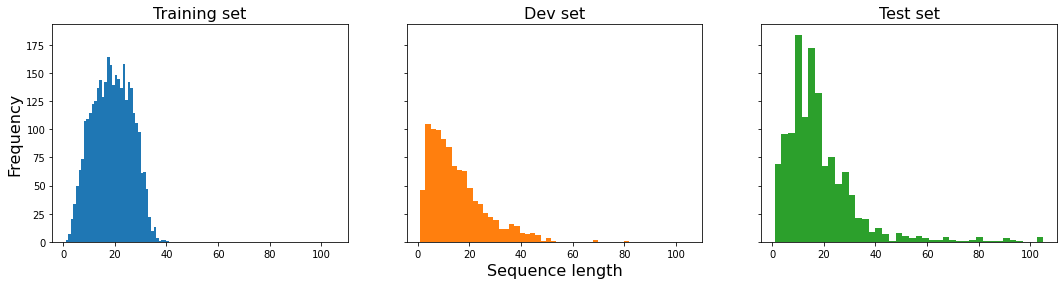
\includegraphics[width=\textwidth]{figs/sequence-lengths-histogram.png}
    \caption{Distributions of the text sequence lengths in the datasets.}
    \label{fig:sequence-lengths}
\end{figure*}

\subsection{Data exploration}

The W-NUT 2017 shared task \citep{derczynski-etal-2017-results} contains contexts mined from various social medias, including Twitter, Reddit, YouTube and StackExchange. Its datasets are encoded in the CoNLL format, where sentences are encoded into multiple rows, each containing the annotation of a word/token, and different sentences are separated by empty rows. The tokens are labelled in a `BIO' format, where `B' (beginning) represents the first word of a named entity, `I' (inside) represents any other word inside a named entity, and `O' (outside) represents a non-named entity word. Furthermore, the named entities are annotated into the following 6 entity types:
\begin{enumerate}[noitemsep]
    \item \texttt{person}
    \item \texttt{location}
    \item \texttt{corporation}
    \item \texttt{product}
    \item \texttt{creative-work}
    \item \texttt{group}
\end{enumerate}

Table \ref{table:entity-counts} shows the numbers of entities found in the training, development and test datasets.

\begin{table}
    \centering
    \begin{tabular}{lrrr}
        \hline 
        \textbf{} & \textbf{Train} & \textbf{Dev} & \textbf{Test} \\
        \hline
        Documents & 3,375 & 993 & 1,283 \\
        Tokens & 62,236 & 15,382 & 23,323 \\
        Entities & 1,964 & 826 & 1,076 \\
        \hline
        \texttt{person} & 655 & 464 & 426 \\
        \texttt{location} & 544 & 74 & 150 \\
        \texttt{corporation} & 221 & 33 & 66 \\
        \texttt{product} & 141 & 112 & 127 \\
        \texttt{creative-work} & 139 & 105 & 142 \\
        \texttt{group} & 264 & 38 & 165 \\
        \hline
    \end{tabular}
    \caption{W-NUT 2017 dataset statistics}
    \label{table:entity-counts}
\end{table}

\subsection{Feature extraction}

Since the goal of the task in this final practical is to maximise the `entity' rather than `surface' performance on the W-NUT 2017 shared task (i.e., there is no need to predict the entity types), I focused on the `BIO only' labels. Firstly, the tokens, the universal PoS (UPoS) tags, and the named entity labels were converted into integers, in order to be fed into the NNs. Then, the format for the datasets were converted from one token per row to one entire text sequence per row, to make them ready for the inputs to the NN classifiers. Since the dimensions of the NNs are pre-defined, all text sequences must carry the same number of tokens, which means all texts must be padded to the longest sequence in the training, development and test datasets. However, this introduces the following problem: while the average length of the text sequences is 17.86 tokens, the longest text sequence is 105 tokens long in the test set, which is clearly an outlier as shown in Figure \ref{fig:sequence-lengths}. This means that almost all the texts are padded with a very long sequence of padding tokens, which are most likely to be even longer than the original text, causing the labels of the datasets to be dominated by the padding label. Finally, in order to prepare the labels as binary values, I converted the label sequences to a one-hot encoding, including an extra index for the `padding' label.

\section{Neural Network Structure}

\subsection{Bidirectional LSTM layer}

LSTM based networks have been proven effective in sequence labelling problems for their capability of balancing both long-term and short-term memories. In a unidirectional LSTM layer, the hidden states only take information from the past, which may be adequate to label an entire sequence (for example, sentiment analysis), but can lose useful information when labelling each token. A bidirectional LSTM (BiLSTM) layer enables its hidden states to capture the information from both the past and the future contexts, which can be particularly helpful in labelling a token. 

Mathematically, a BiLSTM layer takes a sequence of embeddings (feature vectors) for the tokens of the sequence as its input, denoted as $(\bm{x}_1,\cdots,\bm{x}_n)$. The output of the BiLSTM layer is then a sequence of word representations, denoted as $(\bm{y}_1,\cdots,\bm{y}_n)$. For every word embedding $\bm{x}_t$ in a given input sequence, two hidden states $\bm{h}_t^f$ and $\bm{h}_t^b$ are computed from the forward LSTM and the backward LSTM layers, respectively. The final output $\bm{y}_t$ is then the concatenation of the forward $\bm{h}_t^f$ and backward $\bm{h}_t^b$, as shown in the following equations:

$$\begin{aligned}
    \bm{h}_t^f &= \text{LSTM}_\textit{forward}(\bm{x}_t, \bm{h}_{t-1}^f) \\
    \bm{h}_t^b &= \text{LSTM}_\textit{backward}(\bm{x}_t, \bm{h}_{t+1}^f) \\
    \bm{y}_t &= \bm{h}_t^f \oplus \bm{h}_t^b
\end{aligned}$$

The structure of a BiLSTM layer is shown in Figure \ref{fig:BiLSTM}.

\begin{figure}
    \centering
    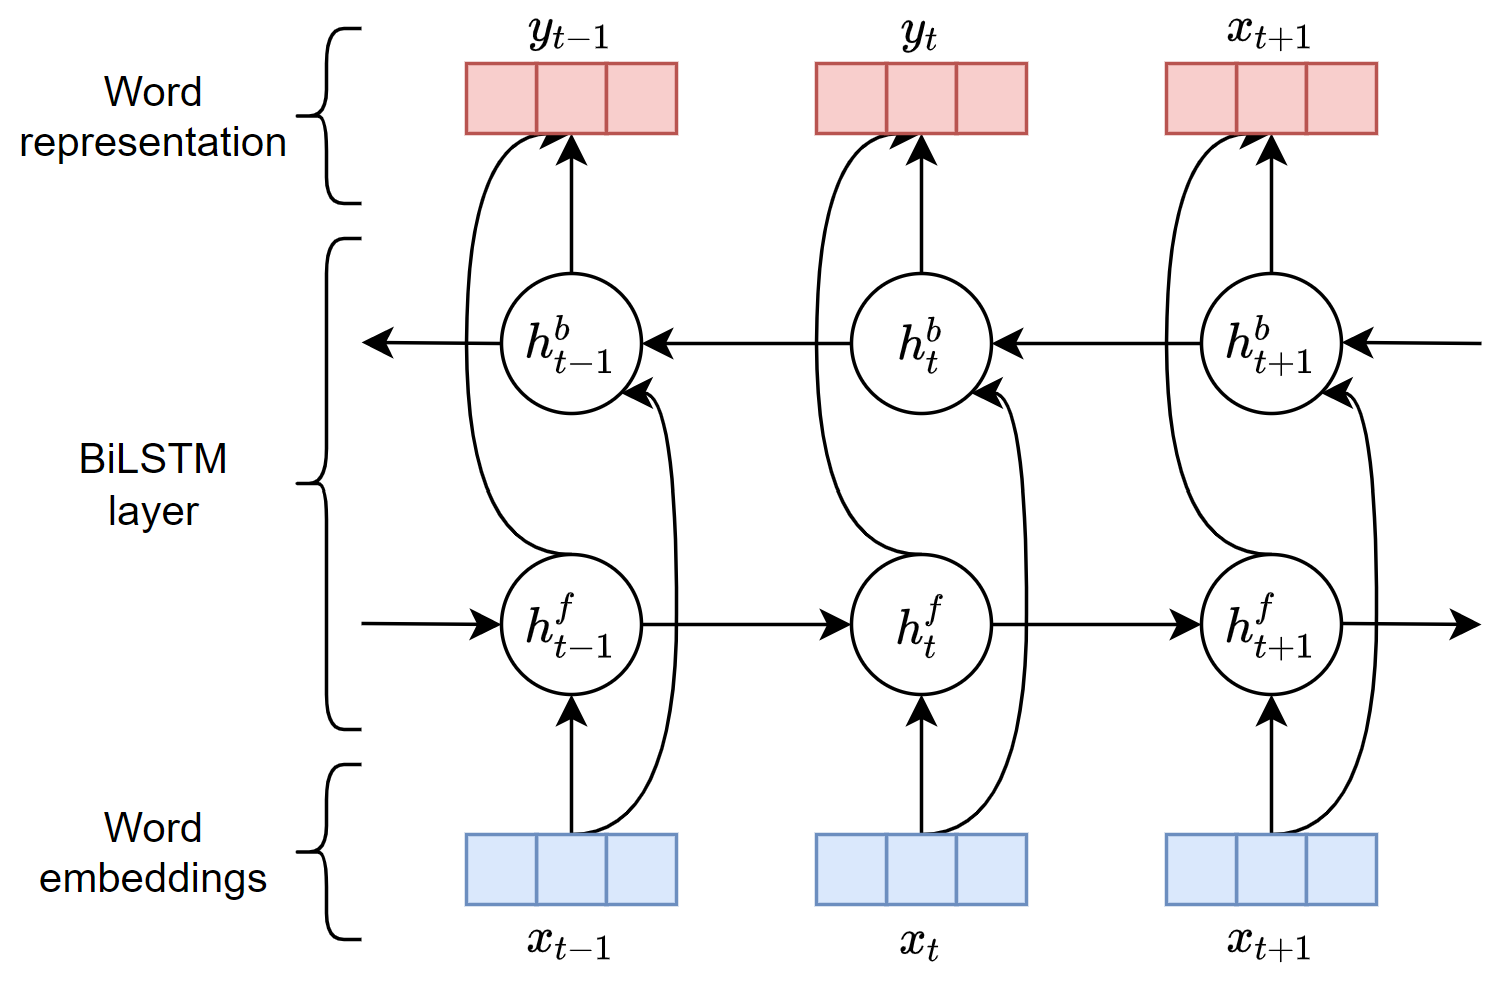
\includegraphics[width=\columnwidth]{figs/BiLSTM.png}
    \caption{Structure of a BiLSTM layer.}
    \label{fig:BiLSTM}
\end{figure}

\subsection{Overall structure}

In this final practical, I adopted the default NN structure provided by the Colab Notebook, which is a sequential model with an embedding layer with an embedding size of 128 for computing the word embeddings, followed by a BiLSTM layer with 50 hidden units, a dropout layer with a dropout rate of 0.5 for regularisation and to prevent over-fitting, and finally a dense layer with softmax activation, as shown in Figure \ref{fig:model}. The choice of the output dimensions is subject to the number of classes the model is intended to predict, which will be further explained in Section \ref{subsection:2class}. Besides, the word embeddings after the embedding layer can also be concatenated with other feature vectors, effectively changing the structure of the model, which will also be elaborated in Section \ref{subsection:PoS}.

\begin{figure}
    \centering
    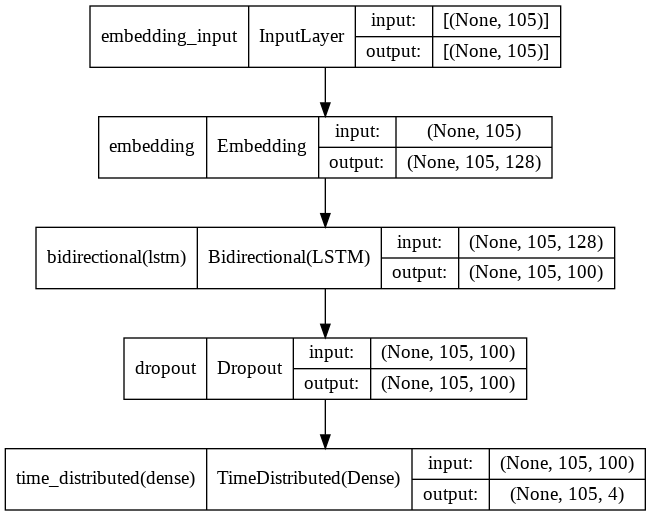
\includegraphics[width=\columnwidth]{figs/model.png}
    \caption{NN structure for the final practical.}
    \label{fig:model}
\end{figure}

\section{Improving Model Performance}

\begin{figure*}
    \centering
    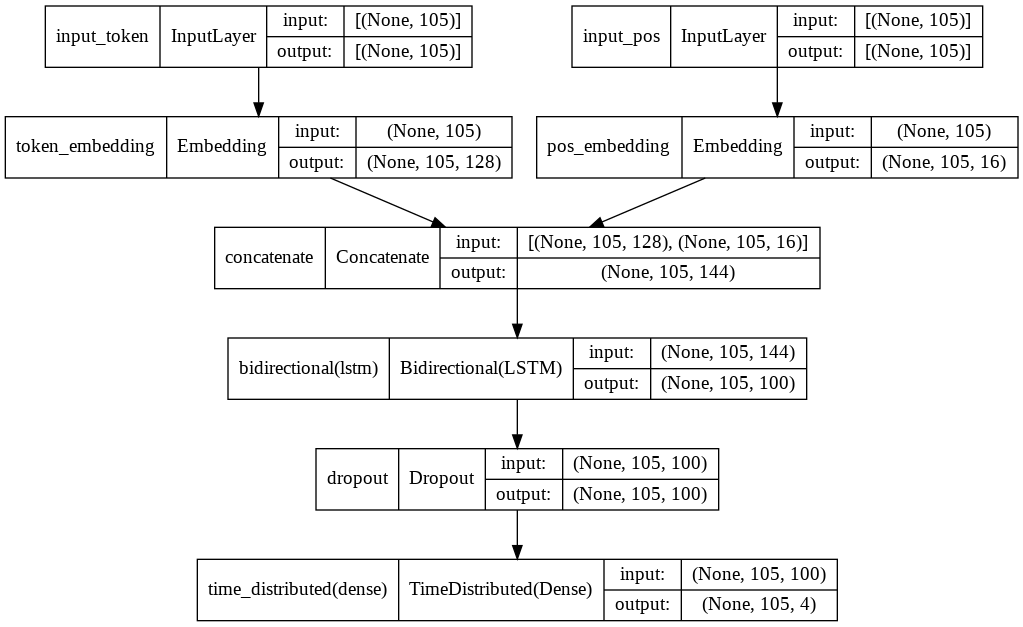
\includegraphics[width=0.733\textwidth]{figs/model-pos.png}
    \caption{NN structure with PoS embeddings appended to the word embeddings.}
    \label{fig:model-pos}
\end{figure*}

Due to the dominant numbers of `outside' and `padding' labels in the training set, the default NN fails to predict any named entity if not combined with any optimisation. However, there are serveral techniques to improve the model's performance by applying extra processing on the training data, without having to change the core structure of the NN. Multiple techniques can also be applied at the same time, in order to further improve the model's performance. 

\subsection{Downweighting non-named entity labels} \label{subsection:downweighting}

Since the labels in the training set are imbalanced, it is useful to assign different weights to the labels, and particularly in this case, to downweigh the non-named entity labels, in order to reduce their importances for the NN's targets. In this final practical, I investigated the downweighting of the `outside' and `padding' labels by multiplying a downweighting ratio to them in the one-hot encoded labels while leaving the named entity labels (i.e., the `beginning' and `inside' labels) unchanged. I have experimented different downweighting ratios ranging from 0.1 to 0.9.

\subsection{Downsampling} \label{subsection:downsampling}

The training set contains a lot of text sequences that do not contain any named entities. By removing those text sequences from the training set, I can effectively perform downsampling on the non-named entity labels, and reduce the gap between the numbers of the named entity labels and the non-named entity labels. However, such downsampling technique has its limitation: even though all text sequences without any named entities have been removed, there are still only a few named entities in each of the remaining text sequences. Consequently, the downsampled training set is still dominated by the `outside' and `padding' labels (only less dominant than the original training set without downsampling), as shown in the label counts in Table \ref{table:downsampled-label-counts}. Downweighting (as aforementioned in Section \ref{subsection:downweighting}) can also be applied together with downsampling, in order to further improve the model's performance.

\begin{table}
    \centering
    \begin{tabular}{rrrrr}
        \hline 
        \textbf{Texts} & \textbf{B} & \textbf{I} & \textbf{O} & \textbf{Padding} \\
        \hline
        1,222 & 1,964 & 1,177 & 22,152 & 103,017 \\
        \hline
    \end{tabular}
    \caption{Label counts of the downsampled training set.}
    \label{table:downsampled-label-counts}
\end{table}

\begin{table}
    \centering
    \resizebox{\columnwidth}{!}{\begin{tabular}{lrrrr}
        \hline 
        \textbf{Dataset} & \textbf{Texts} & \textbf{B-I} & \textbf{O} & \textbf{Padding} \\
        \hline
        Original    & 3,375 & 3,141 & 59,095 & 292,139 \\
        Downsampled & 1,222 & 3,141 & 22,152 & 103,017 \\
        \hline
    \end{tabular}}
    \caption{Label counts of the downsampled training set.}
    \label{table:2class-label-counts}
\end{table}

\subsection{Merging B and I labels} \label{subsection:2class}

In the W-NUT 2017 datasets, the `B' (beginning) label marks the beginning of a named entity, and the `I' (inside) label indicates continuation of that same named entity. However, there is no characteristic difference between the first word of a named entity and the rest of the words of it, and it can be more or less counter-intuitive to separate them as different classes. Therefore, it is sensible to merge these `B' and `I' labels, so that the NER problem becomes a 2-class classification problem (or a 3-class classification problem, if the `padding' label is counted), which makes it easier for an NN to fit. This would require the output dimensions of the NN to be 3 (taking the `padding' label into account) rather than 4 as shown in Figure \ref{fig:model}, and extra post-processing needs to be performed after the model predictions, in order to split the named entity labels back into `B' and `I'. To do this, I set all named entity labels without a preceding named entity label to `B', and all other named entity labels (i.e. the named entity labels whose preceding label is also a named entity) to `I'. Downweighting (as aforementioned in Section \ref{subsection:downweighting}) and downsampling (as aforementioned in Section \ref{subsection:downsampling}) can also be applied together with this techinique, in order to further improve the model's performance. Table \ref{table:2class-label-counts} shows the label counts after merging the `B' and `I' labels, both with and without downsampling.

\subsection{Adding part-of-speech embeddings} \label{subsection:PoS}

PoS is a very important feature in NER. As has been shown in Practical 2, even a na\"{i}ve classifier that identifies all proper nouns as named entities can achieve a F1-score of 44.6\%, which is even higher than a trained feature-based classifier. However, the default NN only takes into account of the word embeddings, which can be considered to be a huge information loss for neglecting the PoS features. Therefore, for this technique, I introduced a embedding layer with an embedding size of 16 to compute the PoS embeddings, and append it to the existing word embeddings. This inevitably changed the structure of the NN, as shown in Figure \ref{fig:model-pos}. Downweighting (as aforementioned in Section \ref{subsection:downweighting}), downsampling (as aforementioned in Section \ref{subsection:downsampling}) and the merging of B and I labels (as aforementioned in Section \ref{subsection:2class}) can also be applied together with this techinique, in order to further improve the model's performance. 

\section{Experiments}

\subsection{Experimental setup}

\paragraph{Training:}
In my final practical, all combinations of the choices of techniques, namely whether to apply downsampling, merging of the named entity labels, and the inclusion of the PoS embeddings, have been assigned with an NN and tried exhaustively, resulting in 8 families of NNs to be trained:
\begin{itemize}[noitemsep]
    \item \textbf{BiLSTM:} the BiLSTM models with no techniques applied other than downweighting of the non-named entity labels;
    \item \textbf{BiLSTM-DS:} the BiLSTM models trained using the downsampled training set;
    \item \textbf{BiLSTM-2Class:} the BiLSTM models with the `B' and `I' labels merged;
    \item \textbf{BiLSTM-2Class-DS:} the BiLSTM models with the `B' and `I' labels merged, and trained using the downsampled trainng set;
    \item \textbf{BiLSTM-PoS:} the BiLSTM models with PoS embeddings;
    \item \textbf{BiLSTM-PoS-DS:} the BiLSTM models with PoS embeddings, and trained using the downsampled trainng set;
    \item \textbf{BiLSTM-PoS-2Class-DS:} the BiLSTM models with PoS embeddings, and merging the `B' and `I' labels;
    \item \textbf{BiLSTM-PoS-2Class-DS:} the BiLSTM models with PoS embeddings, merging the `B' and `I' labels, and trained using the downsampled trainng set.
\end{itemize}
In addition, for each of the NN families, downweighting of the `O' and `padding' labels with downweighting ratios ranging from 0.1 to 0.9 are tried, as well as the no-downweighting options, have been tried, forming 10 different NNs in each family. All NNs were trained using an Adam optimiser with a learning rate of $10^{-3}$, with a batch size of 32. An early stopping criterion is applied, in order to halt training if improvements are not seen after a certain number of epochs. In this final practical, I did not make any attempt on hyperparameter tuning of the NNs, but focused on the data-processing side to improve the model's performance.

\paragraph{Evaluation:}
After all 80 NNs have been trained, I evaluated them on the W-NUT 2017 development and test datasets, using entity precision, recall and F1-score as evaluation metrics. I used the na\"{i}ve classifier introduced in Practical 2 which identifies all proper nouns as named entities as the non-machine learning (ML) baseline, and used both the default feature-based NER classifier provided by Practical 2, and my feature-based NER classifier from Assignment 2\footnote{\href{https://colab.research.google.com/drive/1NFr1gBZZX6JvxzVIanZuLs-uS6ddGJUM?usp=sharing}{Colab Notebook}}, as the non-NN ML baseline. I also used the BiLSTM model without any techniques (i.e. the default BiLSTM model provided in the final practical) as the NN baseline. The evaluation results are analysed in the next section.

\subsection{Results}

The evaluation results of my trained NNs are reported in Table \ref{table:eval-results} and \ref{table:eval-results-pos} in Appendix \ref{appendix}. The result shows that almost all NNs struggled to catch up with the baseline performance, with the BiLSTM model applied with all the techniques (i.e., PoS embeddings, merging the named entity labels, downsampling, and downweighting of ratio 0.2) simultaneously being the only exception. Besides, only the best models in the BiLSTM-PoS plus at least one extra optimisation technique in merging the named entity labels and downsampling families can outperform the feature-based baseline.

As of the downweighting technique, nearly all NN families preferred the lowest downweighting ratio (0.1), except the BiLSTM-PoS-2Class-DS family that peaked at 0.2. All NN families demonstrated a clear increase in the performance as the downweighting ratio becomes smaller, and most of the NN families failed to predict any named entity, except the BiLSTM-2Class and BiLSTM-PoS-2Class-DS families, when there was no downweighting applied. In general, the BiLSTM models with PoS embeddings react less to downweighting, when the downweighting ratio is not small enough.

Other than downweighting, which is almost the necessary component required for making the NNs predict useful results at all, the PoS embedding shows the most significant improvement on the NN's performance, which coincides with my hypothesis at the beginning. The downsampling technique and the merging of named entity labels showed no particular difference in the improvement on performance when applied alone, but can also show a great improvement on the performance when combined together. There is also no conflict between any pair of optimisation techniques -- they always produce better results when combined together.

When analysing the precision and recall of the models, it can be seen that in most cases the precision can be a lot higher than the recall, showing that the named entities predicted by the NNs are more likely to be actual named entities, compared to the probability of the NNs predicting named entities when the tokens are actually named entities. This can also be due to the dominant number of non-named entity (`outside' and `padding') labels, causing the NNs to predict named entities only when they are absolutely confident.

The best performing NN produced in my final practical is the BiLSTM model with PoS embeddings, merging the named entity labels, trained with the downsampled training set, with downweighting of the non-named entity labels of a downweighting ratio 0.2. It achieved a F1-score of 36.3\%, which is the highest in all models, including the selected baselines.

\section{Conclusion}

In this final practical, I investigated the NN structure provided by the Colab Notebook, and performed appropriate data exploration and feature extraction for the NER task. I have also explored several data-processing techniques in order to improve the NN's performance, namely downweighting non-named entity labels, downsampling, merging named entity labels, and adding part-of-speech (PoS) embeddings. I evaluated my trained models on the W-NUT 2017 development and test sets, using entity precision, recall and F1-score as evaluation metrics, obtaining the best F1-score of 36.3\% from a BiLSTM model with PoS embeddings, merging the named entity labels, trained with the downsampled training set, with downweighting of the non-named entity labels of a downweighting ratio 0.2. The results show that an arbitrarily designed NN can struggle in the NER task and can be outperformed by non-NN ML approaches or even non-ML approaches, which means that NNs are certainly not the almighty solution to NLP problems, unless with very careful and fine-grained design. However, it is delightful to see that even with a poorly designed NN structure and no hyperparameter tuning, it is still possible to achieve significant improvements on the performance, by detailed investigations into the dataset and combinations of suitable optimisation techniques in data processing.

\bibliography{anthology}
\bibliographystyle{acl_natbib}

\appendix
\section{Appendix: Model Performances (See Next Page)} \label{appendix}

\begin{table*}
    \centering
    \begin{tabular}{lrrrrrr}
        \hline
        \multirow{2}{*}{\textbf{Model}} & \multicolumn{3}{c}{\textbf{Dev set}} & \multicolumn{3}{c}{\textbf{Test set}} \\
        \cline{2-7}
        {} & \textbf{Precision} & \textbf{Recall} & \textbf{F1} & \textbf{Precision} & \textbf{Recall} & \textbf{F1} \\
        \hline
        Baseline (PROPN) & \textcolor{Green}{\textbf{44.3\%}} & \textcolor{Green}{\textbf{44.9\%}} & \textcolor{Green}{\textbf{44.6\%}} & \textcolor{Green}{\textbf{30.7\%}} & 42.6\% & \textcolor{Green}{\textbf{35.7\%}} \\
        \hline
        Feature-based (Practical 2)  & 18.7\% & \textcolor{Green}{\textbf{44.9\%}} & 26.4\% & 15.2\% & \textcolor{Green}{\textbf{44.9\%}} & 22.7\% \\
        Feature-based (Assignment 2) & \textbf{27.5\%} & 44.3\% & \textbf{34.0\%} & \textbf{20.4\%} & 44.7\% & \textbf{28.0\%} \\
        \hline
        BiLSTM & 0.0\% & 0.0\% & 0.0\% & 0.0\% & 0.0\% & 0.0\% \\
        \hline
        BiLSTM-DW\textsubscript{0.9} &  0.0\% &  0.0\% &  0.0\% &  0.0\% &  0.0\% &  0.0\% \\
        BiLSTM-DW\textsubscript{0.8} &  0.0\% &  0.0\% &  0.0\% &  7.1\% &  0.1\% &  0.2\% \\
        BiLSTM-DW\textsubscript{0.7} &  0.0\% &  0.0\% &  0.0\% &  8.3\% &  0.2\% &  0.4\% \\
        BiLSTM-DW\textsubscript{0.6} &  8.3\% &  0.1\% &  0.2\% &  6.4\% &  0.3\% &  0.5\% \\
        BiLSTM-DW\textsubscript{0.5} & \textbf{21.4\%} &  0.7\% &  1.4\% &  6.5\% &  0.5\% &  0.9\% \\
        BiLSTM-DW\textsubscript{0.4} &  0.0\% &  0.0\% &  0.0\% &  0.0\% &  0.0\% &  0.0\% \\
        BiLSTM-DW\textsubscript{0.3} & 20.0\% &  0.1\% &  0.2\% &  0.0\% &  0.0\% &  0.0\% \\
        BiLSTM-DW\textsubscript{0.2} &  2.9\% &  0.1\% &  0.2\% &  6.0\% &  1.4\% &  2.3\% \\
        BiLSTM-DW\textsubscript{0.1} & 16.6\% &  \textbf{8.4\%} & \textbf{11.1\%} & \textbf{13.1\%} & \textbf{11.5\%} & \textbf{12.2\%} \\
        \hline
        BiLSTM-DS & 0.0\% & 0.0\% & 0.0\% & 0.0\% & 0.0\% & 0.0\% \\
        BiLSTM-DS-DW\textsubscript{0.9} &  0.0\% &  0.0\% &  0.0\% &  0.0\% &  0.0\% &  0.0\% \\
        BiLSTM-DS-DW\textsubscript{0.8} &  0.0\% &  0.0\% &  0.0\% &  0.0\% &  0.0\% &  0.0\% \\
        BiLSTM-DS-DW\textsubscript{0.7} & \textbf{25.0\%} &  0.1\% &  0.2\% &  0.0\% &  0.0\% &  0.0\% \\
        BiLSTM-DS-DW\textsubscript{0.6} &  7.1\% &  0.1\% &  0.2\% &  2.0\% &  0.1\% &  0.2\% \\
        BiLSTM-DS-DW\textsubscript{0.5} &  6.5\% &  0.4\% &  0.7\% &  1.5\% &  0.2\% &  0.3\% \\
        BiLSTM-DS-DW\textsubscript{0.4} & 15.3\% &  2.1\% &  3.6\% &  5.6\% &  1.4\% &  2.2\% \\
        BiLSTM-DS-DW\textsubscript{0.3} & 14.6\% &  4.4\% &  6.7\% &  7.7\% &  4.5\% &  5.6\% \\
        BiLSTM-DS-DW\textsubscript{0.2} & 10.9\% &  8.8\% &  9.7\% &  7.4\% & 10.4\% & 8.7\% \\
        BiLSTM-DS-DW\textsubscript{0.1} & 15.9\% & \textbf{34.3\%} & \textbf{21.7\%} & \textbf{10.1\%} & \textbf{31.4\%} & \textbf{15.3\%} \\
        \hline
        BiLSTM-2Class & 20.0\% & 0.1\% & 0.2\% & 12.5\% &  0.2\% &  0.4\% \\
        BiLSTM-2Class-DW\textsubscript{0.9} & \textbf{31.2\%} &  0.6\% &  1.2\% & 11.4\% &  0.4\% &  0.7\% \\
        BiLSTM-2Class-DW\textsubscript{0.8} & 26.3\% &  1.2\% &  2.4\% & 12.7\% &  0.7\% &  1.2\% \\
        BiLSTM-2Class-DW\textsubscript{0.7} & 24.1\% &  1.6\% &  3.0\% & 13.7\% &  1.2\% &  2.2\% \\
        BiLSTM-2Class-DW\textsubscript{0.6} & 29.5\% &  2.9\% &  5.2\% & \textbf{18.4\%} &  2.3\% &  4.2\% \\
        BiLSTM-2Class-DW\textsubscript{0.5} &  0.0\% &  0.0\% &  0.0\% &  0.0\% &  0.0\% &  0.0\% \\
        BiLSTM-2Class-DW\textsubscript{0.4} &  3.4\% &  0.1\% &  0.2\% &  6.4\% &  0.6\% &  1.0\% \\
        BiLSTM-2Class-DW\textsubscript{0.3} & 13.0\% &  1.7\% &  3.1\% &  7.1\% &  2.8\% &  4.0\% \\
        BiLSTM-2Class-DW\textsubscript{0.2} & 18.7\% &  9.1\% & 12.2\% &  9.1\% &  9.7\% &  9.4\% \\
        BiLSTM-2Class-DW\textsubscript{0.1} & 23.4\% & \textbf{20.6\%} & \textbf{21.9\%} & 15.2\% & \textbf{22.2\%} & \textbf{18.0\%} \\
        \hline
        BiLSTM-2Class-DS & 0.0\% & 0.0\% & 0.0\% & 1.9\% & 0.1\% & 0.2\% \\
        BiLSTM-2Class-DS-DW\textsubscript{0.9} & 12.3\% &  0.9\% &  1.6\% &  2.6\% &  0.3\% &  0.5\% \\
        BiLSTM-2Class-DS-DW\textsubscript{0.8} & 15.5\% &  2.1\% &  3.7\% &  9.2\% &  2.3\% &  3.7\% \\
        BiLSTM-2Class-DS-DW\textsubscript{0.7} & 15.7\% &  3.6\% &  5.9\% & 10.2\% &  4.0\% &  5.8\% \\
        BiLSTM-2Class-DS-DW\textsubscript{0.6} & 19.0\% &  7.3\% & 10.6\% &  9.9\% &  5.7\% &  7.2\% \\
        BiLSTM-2Class-DS-DW\textsubscript{0.5} & 20.3\% & 11.3\% & 14.5\% & 11.8\% & 10.0\% & 10.9\% \\
        BiLSTM-2Class-DS-DW\textsubscript{0.4} & 20.5\% & 17.4\% & 18.8\% & 10.5\% & 13.2\% & 11.7\% \\
        BiLSTM-2Class-DS-DW\textsubscript{0.3} & 19.8\% & 24.2\% & 21.8\% & 12.1\% & 21.5\% & 15.5\% \\
        BiLSTM-2Class-DS-DW\textsubscript{0.2} & \textbf{20.8\%} & 29.9\% & 24.5\% & \textbf{13.5\%} & 28.1\% & 18.2\% \\
        BiLSTM-2Class-DS-DW\textsubscript{0.1} & 19.3\% & \textbf{40.4\%} & \textbf{26.1\%} & 12.7\% & \textbf{36.1\%} & \textbf{18.8\%} \\
        \hline
    \end{tabular}
    \caption{Evaluation results of the word-embeddings-only models on the dev test sets (here DW represents downweighting, DS represents downsampling, and 2Class represents merging B and I labels).}
    \label{table:eval-results}
\end{table*}

\begin{table*}
    \centering
    \begin{tabular}{lrrrrrr}
        \hline
        \multirow{2}{*}{\textbf{Model}} & \multicolumn{3}{c}{\textbf{Dev set}} & \multicolumn{3}{c}{\textbf{Test set}} \\
        \cline{2-7}
        {} & \textbf{Precision} & \textbf{Recall} & \textbf{F1} & \textbf{Precision} & \textbf{Recall} & \textbf{F1} \\
        \hline
        Baseline (PROPN) & \textcolor{Green}{\textbf{44.3\%}} & \textcolor{Green}{\textbf{44.9\%}} & \textcolor{Green}{\textbf{44.6\%}} & 30.7\% & 42.6\% & 35.7\% \\
        \hline
        Feature-based (Practical 2)  & 18.7\% & \textbf{44.9\%} & 26.4\% & 15.2\% & \textcolor{Green}{\textbf{44.9\%}} & 22.7\% \\
        Feature-based (Assignment 2) & \textbf{27.5\%} & 44.3\% & \textbf{34.0\%} & \textbf{20.4\%} & 44.7\% & \textbf{28.0\%} \\
        \hline
        BiLSTM-PoS & 0.0\% & 0.0\% & 0.0\% & 0.0\% & 0.0\% & 0.0\% \\
        BiLSTM-PoS-DW\textsubscript{0.9} &  0.0\% &  0.0\% &  0.0\% &  0.0\% &  0.0\% &  0.0\% \\
        BiLSTM-PoS-DW\textsubscript{0.8} &  0.0\% &  0.0\% &  0.0\% &  0.0\% &  0.0\% &  0.0\% \\
        BiLSTM-PoS-DW\textsubscript{0.7} &  0.0\% &  0.0\% &  0.0\% &  0.0\% &  0.0\% &  0.0\% \\
        BiLSTM-PoS-DW\textsubscript{0.6} &  0.0\% &  0.0\% &  0.0\% &  0.0\% &  0.0\% &  0.0\% \\
        BiLSTM-PoS-DW\textsubscript{0.5} &  0.0\% &  0.0\% &  0.0\% &  0.0\% &  0.0\% &  0.0\% \\
        BiLSTM-PoS-DW\textsubscript{0.4} &  0.0\% &  0.0\% &  0.0\% &  2.9\% &  0.1\% &  0.2\% \\
        BiLSTM-PoS-DW\textsubscript{0.3} & 25.7\% &  1.1\% &  2.1\% &  5.7\% &  0.8\% &  1.5\% \\
        BiLSTM-PoS-DW\textsubscript{0.2} & 22.4\% &  5.9\% &  9.4\% & 15.6\% &  9.7\% & 11.9\% \\
        BiLSTM-PoS-DW\textsubscript{0.1} & \textbf{31.5\%} & \textbf{31.7\%} & \textbf{31.6\%} & \textbf{19.9\%} & \textbf{31.7\%} & \textbf{24.4\%} \\
        \hline
        BiLSTM-PoS-DS & 0.0\% & 0.0\% & 0.0\% & 0.0\% & 0.0\% & 0.0\% \\
        BiLSTM-PoS-DS-DW\textsubscript{0.9} &  0.0\% &  0.0\% &  0.0\% &  0.0\% &  0.0\% &  0.0\% \\
        BiLSTM-PoS-DS-DW\textsubscript{0.8} &  0.0\% &  0.0\% &  0.0\% &  3.8\% &  0.1\% &  0.2\% \\
        BiLSTM-PoS-DS-DW\textsubscript{0.7} & 19.2\% &  0.6\% &  1.2\% &  1.6\% &  0.1\% &  0.2\% \\
        BiLSTM-PoS-DS-DW\textsubscript{0.6} & 12.3\% &  1.1\% &  2.0\% &  6.4\% &  1.1\% &  1.9\% \\
        BiLSTM-PoS-DS-DW\textsubscript{0.5} & 16.0\% &  3.0\% &  5.1\% & 11.0\% &  3.8\% &  5.7\% \\
        BiLSTM-PoS-DS-DW\textsubscript{0.4} & 23.9\% & 11.1\% & 15.2\% & 17.4\% & 11.3\% & 13.7\% \\
        BiLSTM-PoS-DS-DW\textsubscript{0.3} & \textbf{33.5\%} & 27.7\% & 30.3\% & 24.9\% & 25.2\% & 25.0\% \\
        BiLSTM-PoS-DS-DW\textsubscript{0.2} & 33.1\% & 35.0\% & 34.0\% & \textbf{26.9\%} & 33.6\% & 29.9\% \\
        BiLSTM-PoS-DS-DW\textsubscript{0.1} & 31.5\% & \textbf{43.8\%} & \textbf{36.7\%} & 24.1\% & \textbf{40.1\%} & \textbf{30.1\%} \\
        \hline
        BiLSTM-PoS-2Class & 0.0\% & 0.0\% & 0.0\% & 0.0\% & 0.0\% & 0.0\% \\
        BiLSTM-PoS-2Class-DW\textsubscript{0.9} &  0.0\% &  0.0\% &  0.0\% &  0.0\% &  0.0\% &  0.0\% \\
        BiLSTM-PoS-2Class-DW\textsubscript{0.8} &  0.0\% &  0.0\% &  0.0\% &  0.0\% &  0.0\% &  0.0\% \\
        BiLSTM-PoS-2Class-DW\textsubscript{0.7} &  0.0\% &  0.0\% &  0.0\% &  4.2\% &  0.1\% &  0.2\% \\
        BiLSTM-PoS-2Class-DW\textsubscript{0.6} & 16.7\% &  0.2\% &  0.5\% & 12.3\% &  0.7\% &  1.2\% \\
        BiLSTM-PoS-2Class-DW\textsubscript{0.5} & 21.7\% &  1.2\% &  2.4\% & 17.7\% &  2.4\% &  4.3\% \\
        BiLSTM-PoS-2Class-DW\textsubscript{0.4} & 37.5\% &  5.2\% &  9.2\% & 27.9\% &  8.9\% & 13.5\% \\
        BiLSTM-PoS-2Class-DW\textsubscript{0.3} & 39.5\% & 13.3\% & 19.9\% & 29.3\% & 17.5\% & 21.9\% \\
        BiLSTM-PoS-2Class-DW\textsubscript{0.2} & \textbf{41.5\%} & 26.7\% & 32.5\% & \textbf{29.4\%} & 28.2\% & 28.8\% \\
        BiLSTM-PoS-2Class-DW\textsubscript{0.1} & 41.2\% & \textbf{42.2\%} & \textbf{41.7\%} & 26.0\% & \textbf{35.4\%} & \textbf{30.0\%} \\
        \hline
        BiLSTM-PoS-2Class-DS & 17.4\% & 1.5\% & 2.7\% & 18.0\% & 2.7\% & 4.7\% \\
        BiLSTM-PoS-2Class-DS-DW\textsubscript{0.9} & 18.6\% &  2.6\% &  4.6\% & 18.7\% &  4.1\% &  6.8\% \\
        BiLSTM-PoS-2Class-DS-DW\textsubscript{0.8} & 27.5\% &  5.8\% &  9.6\% & 22.4\% &  6.8\% & 10.5\% \\
        BiLSTM-PoS-2Class-DS-DW\textsubscript{0.7} & 29.5\% &  8.2\% & 12.8\% & 24.2\% &  9.8\% & 14.0\% \\
        BiLSTM-PoS-2Class-DS-DW\textsubscript{0.6} & 33.0\% & 13.7\% & 19.3\% & 26.2\% & 14.4\% & 18.6\% \\
        BiLSTM-PoS-2Class-DS-DW\textsubscript{0.5} & 39.0\% & 23.2\% & 29.1\% & 29.9\% & 22.8\% & 25.9\% \\
        BiLSTM-PoS-2Class-DS-DW\textsubscript{0.4} & 42.2\% & 33.8\% & 37.5\% & 32.7\% & 32.7\% & 32.7\% \\
        BiLSTM-PoS-2Class-DS-DW\textsubscript{0.3} & \textbf{43.0\%} & 40.6\% & 41.8\% & \textcolor{Green}{\textbf{32.9\%}} & 40.1\% & 36.1\% \\
        BiLSTM-PoS-2Class-DS-DW\textsubscript{0.2} & 40.8\% & \textbf{44.3\%} & \textbf{42.5\%} & 30.8\% & \textbf{44.2\%} & \textcolor{Green}{\textbf{36.3\%}} \\
        BiLSTM-PoS-2Class-DS-DW\textsubscript{0.1} & 36.3\% & 44.0\% & 39.8\% & 27.5\% & 42.7\% & 33.4\% \\
        \hline
    \end{tabular}
    \caption{Evaluation results of the models with PoS embeddings concatenated on the dev test sets.}
    \label{table:eval-results-pos}
\end{table*}

\end{document}
